%%%%%%%%%%%%% Figure 1: PRISMA Chart code
%%%%%%%% Latex code
% % % % % % % % % % % % % % % % % % % % % % % %
%%%%%%%%%%%%%%%%%%%%%%%%%%%%%%%%%
\documentclass[10pt,letterpaper]{article}
\usepackage[top=0.85in,left=2.75in,footskip=0.75in]{geometry}
% amsmath and amssymb packages, useful for mathematical formulas and symbols
\usepackage{amsmath,amssymb}
% Use adjustwidth environment to exceed column width (see example table in text)
\usepackage{changepage}
% textcomp package and marvosym package for additional characters
\usepackage{textcomp,marvosym}
% cite package, to clean up citations in the main text. Do not remove.
\usepackage{cite}
% Use nameref to cite supporting information files (see Supporting Information section for more info)
\usepackage{nameref,hyperref}
\usepackage[right]{lineno}
\usepackage[nopatch=eqnum]{microtype}
\DisableLigatures[f]{encoding = *, family = * }
\usepackage[table]{xcolor}
\usepackage{array}
% create "+" rule type for thick vertical lines
\newcolumntype{+}{!{\vrule width 2pt}}
\newlength\savedwidth
\newcommand\thickcline[1]{%
  \noalign{\global\savedwidth\arrayrulewidth\global\arrayrulewidth 2pt}%
  \cline{#1}%
  \noalign{\vskip\arrayrulewidth}%
  \noalign{\global\arrayrulewidth\savedwidth}%
}
\newcommand\thickhline{\noalign{\global\savedwidth\arrayrulewidth\global\arrayrulewidth 2pt}%
\hline
\noalign{\global\arrayrulewidth\savedwidth}}
% Remove comment for double spacing
%\usepackage{setspace} 
%\doublespacing
% Text layout
\raggedright
\setlength{\parindent}{0.5cm}
\textwidth 5.25in 
\textheight 8.75in

% Bold the 'Figure #' in the caption and separate it from the title/caption with a period
% Captions will be left justified
\usepackage[aboveskip=1pt,labelfont=bf,labelsep=period,justification=raggedright,singlelinecheck=off]{caption}
\renewcommand{\figurename}{Fig}

%%%%%%%%%%%%%%%%%%%%%%%%%%%%%%%%%%%%%%%%%%%%%
% Use the PLoS-provided BiBTeX style
% \bibliographystyle{plos2015}

\usepackage[numbers,sort&compress]{natbib}

% Remove brackets from numbering in List of References
\makeatletter
\renewcommand{\@biblabel}[1]{\quad#1.}
\makeatother

% Header and Footer with logo
\usepackage{lastpage,fancyhdr,graphicx}
\usepackage{epstopdf}

%\pagestyle{myheadings}
%\pagestyle{fancy}
%\fancyhf{}

%\setlength{\headheight}{27.023pt}
%\lhead{\includegraphics[width=2.0in]{PLOS-submission.eps}}
%\rfoot{\thepage/\pageref{LastPage}}
%\renewcommand{\headrulewidth}{0pt}
%\renewcommand{\footrule}{\hrule height 2pt \vspace{2mm}}
\fancyheadoffset[L]{2.25in}
\fancyfootoffset[L]{2.25in}
%\lfoot{\today}

%% Include all macros below

\usepackage{hyperref}
\usepackage{array}
%%%%%%%%%%%%%%%%%%%%%%%%%%%%%%%%%%%%%%%%%%%%%%%%%%
\usepackage{tikz}
\usetikzlibrary{positioning,chains}
\usepackage{float}
% \usepackage{ulem}
\usepackage{array} % Add the array package
\newcolumntype{R}[1]{>{\raggedleft\arraybackslash}p{#1}}
\usepackage{multirow}
% \addbibresource{270_Rayyan_Included.bib} %Imports bibliography file
%\addbibresource{main_references.bib}
% \addbibresource{supplementary_references.bib}
\usepackage{longtable} % For tables that span multiple pages
\usepackage{changepage} % for adjustwidth environment
%%%%%%%%%%%%%%%%%%%%%%%%%%%%%%%%%%%%%%%%%%%%%
%  \usepackage{graphicx}
%\usepackage{tikz}
%\usetikzlibrary{shapes,positioning}
%\usetikzlibrary{shapes,positioning, arrows.meta, matrix}
%\usetikzlibrary{shapes,positioning, arrows.meta, matrix, fit}
\usetikzlibrary{calc}
%\usepackage{listings}
%\usepackage{multicol}
\usepackage{mathtools}
\usepackage{xcolor}
\usepackage{setspace}
\usepackage{subcaption} % Use subcaption instead of subfigure
% \usepackage{subfigure}
% \usepackage{changepage}
\usepackage{lscape} % to enable landscape pages
%%%%%%%%%%%%%%%%%%%%%%%%%%%%%%%%%ttttttttttt
\usepackage{booktabs}
%\addbibresource{270_Rayyan_Included.bib}
% Define a custom command to cite authors without adding to the bibliography
%\newcommand{\citeauthorsilent}[1]{%
%  \citefield{#1}{author}%
%}
%% END MACROS SECTION
%%%%%%%%%%%%%%%%%%%%%%%%%%%%%
%%%%%%%%%%%%%%%%%%%%%%%%%%%%%% Begine document 
\begin{document}
\vspace*{0.2in}
%%%%%%%%%%%%%%%%%%%%%%%%%%%%%%%%%%%%%%%%%%
%\begin{adjustwidth}{-2.0in}{0.1in} % Comment out/remove the adjustwidth environment if the table fits in the text column.
 % Note for Tsega: end of the adjustwidth is before the PRISMA figure 
%%%%%%%%%%%%%%%%%%%%%%%%%%%%%%%%%% % Title must be 250 characters or less.
%\begin{flushleft}
%{\Large
%\textbf\newline{\bf Modelling the impact of behavioural interventions during pandemics: A systematic review % \\ \textbf{Task 2.3– Assessing the Impact of Behavioral Interventions}
%} % Please use "sentence case" for title and headings.
%}
%\newline
%\\
%Tsega Kahsay Gebretekle\textsuperscript{1*} and
%Marijn de Bruin\textsuperscript{2},
%Luc Coffeng\textsuperscript{3},
%Sake de Vlas\textsuperscript{3},
%Peter Lugtig\textsuperscript{4} and 
%[possibly co-authors (to be discussed) and]
%Casper Albers\textsuperscript{1}
%\\
%\bigskip
%\textbf{1} Department of Psychometrics \& Statistics, University of Groningen, The Netherlands
% \\
% \textbf{2} Radboud Medical Center Nijmegen, The Netherlands 
% \\
% \textbf{3} Department of Public Health, Erasmus Medical Center Rotterdam, The Netherlands
% \\
% \textbf{4} Department of Methods \& Statistics, Utrecht University, The Netherlands
% \\
%\bigskip
% Use the asterisk to denote the corresponding authorship.
%* t.k.gebretekle@rug.nl
%\end{flushleft}
%%%%%%%%%%%%%%%%%%%%%%%%%   % abstract below 300 words
%\section*{ABSTRACT}

%\newpage

\begin{minipage}{0.6\textwidth}
    \begin{adjustwidth}{-2.25in}{0in}
        %%%%%%%%% here
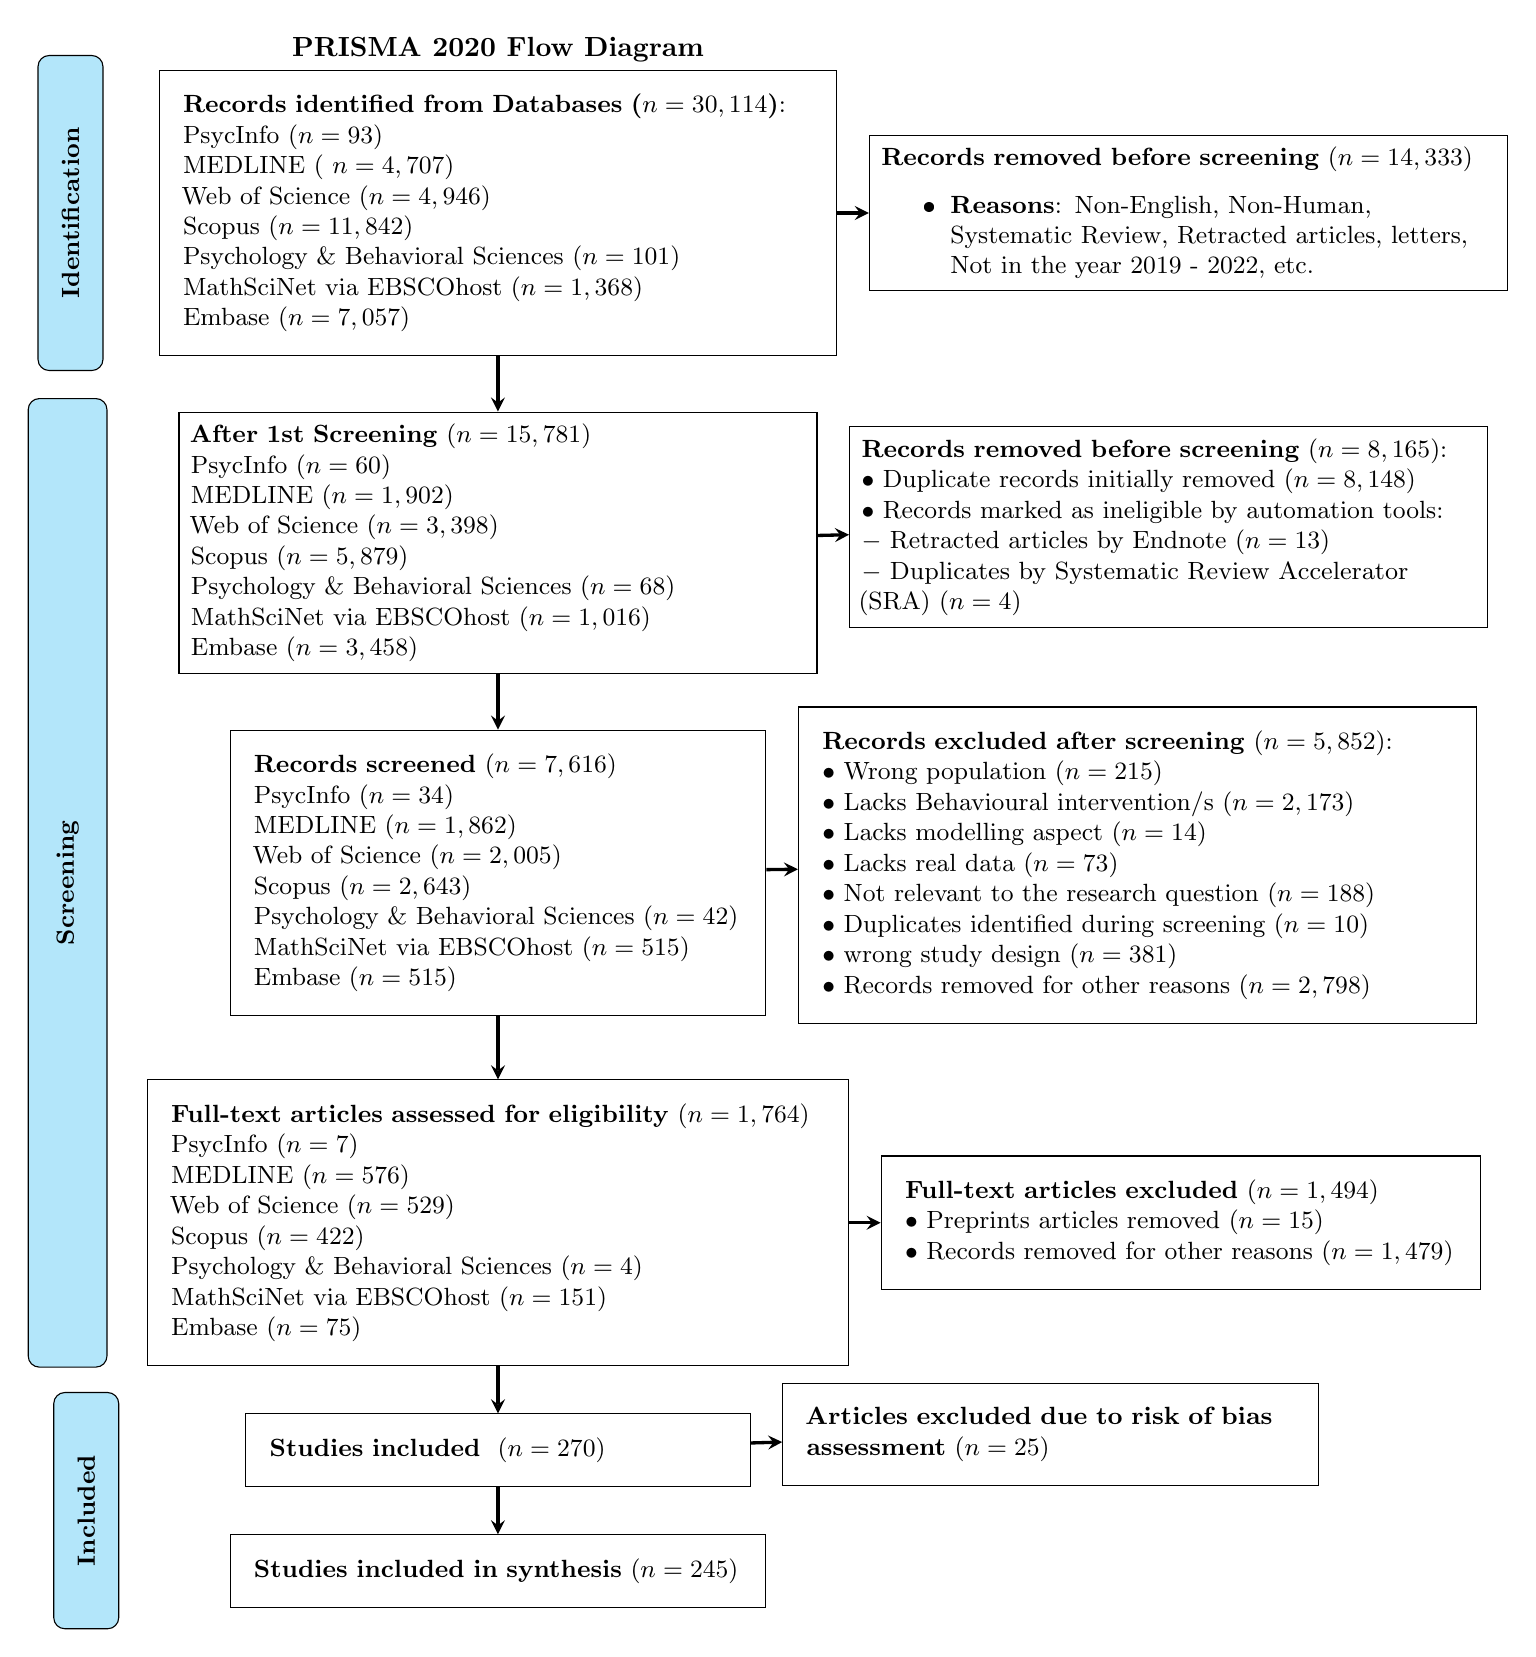
\begin{tikzpicture}[
  node distance=8mm and 4mm,
  start chain=going below,
  mynode/.style={draw, rectangle, align=left, text width=8cm, font=\small, inner sep=2ex, on chain},
   mynode1/.style={draw, rectangle, align=left, text width=7.8cm, font=\small, inner sep=1ex, on chain},
  mynode2/.style={draw, rectangle, align=left, text width=6.2cm, font=\small, inner sep=2ex, on chain},
  mynode1full/.style={draw, rectangle, align=left, text width=7cm, font=\small, inner sep=2ex, on chain},
   mynode4/.style={draw, rectangle, align=left, text width=8.3cm, font=\small, inner sep=2ex, on chain},
    mynode5/.style={draw, rectangle, align=left, text width=5.8cm, font=\small, inner sep=2ex, on chain},
  mylabel/.style={draw, rectangle, align=center, rounded corners, font=\small\bfseries, inner sep=2ex, fill=cyan!30, minimum height=40mm, on chain},
  mylabel2/.style={draw, rectangle, align=center, rounded corners, font=\small\bfseries, inner sep=2ex, fill=cyan!30, minimum height=3cm, on chain},
  every join/.style=arrow, arrow/.style={very thick,-stealth},
  largeLabel/.style={mylabel, minimum height=12.3cm, minimum width=1cm },
     %shortLabel/.style={mylabel, minimum height=4cm, minimum width=2cm },
     myshortnode/.style={draw, rectangle, align=left, text width=6cm, font=\small, inner sep=1ex, on chain},
     mytitlenode/.style = {draw, rectangle, align=center, text width=8cm,font=\bfseries, inner sep=2ex},
]
\coordinate (tc);
\node[ above=of tc, yshift=10mm, font=\bfseries, node distance=25mm] {PRISMA 2020 Flow Diagram};
% box 1
% Leftmost chain (Records identified from)
\node (n1a) [mynode] {\textbf{Records identified from Databases ($n= 30,114$)}:\\  PsycInfo ($n=93$)\\ MEDLINE ( $n=4,707$)\\
Web of Science ($n=4,946$)\\ Scopus ($n=11,842$) \\ Psychology \& Behavioral Sciences ($n=101$)\\
MathSciNet via EBSCOhost ($n=1,368$)\\Embase ($n=7,057$)};
% box 2
% Rightmost chain (Records removed)
\node (n1b) [mynode1, right=of n1a, node distance=20mm] {\textbf{Records removed before screening} ($n=14,333$)\\
\begin{itemize}
    \item \textbf{Reasons}: Non-English, Non-Human, Systematic Review, Retracted articles, letters, Not in the year 2019 - 2022, etc.
\end{itemize} };
%%%%%%%%%%%%%%%%%%%%%%%%%%%%%%%%%% After duplicate 
\node (n2a) [mynode1, below=of n1a,yshift=1mm] {\textbf{After 1st Screening} ($n=15,781$)\\PsycInfo ($n=60$)\\ MEDLINE ($n=1,902$)\\
Web of Science ($n=3,398$)\\ Scopus ($n=5,879$) \\ Psychology \& Behavioral Sciences ($n=68$)\\
MathSciNet via EBSCOhost ($n=1,016$)\\Embase ($n=3,458$) 
};
\node (n2b) [mynode1, right=of n2a, node distance=20mm,yshift=2mm] {\textbf{Records removed before screening} ($n=8,165$): \\ $ \bullet$ Duplicate records initially removed ($n=8,148$) \\ $ \bullet$ Records marked as ineligible by automation tools:  \\ $ - $ Retracted articles by Endnote ($n=13$) \\ $-$ Duplicates by Systematic Review Accelerator (SRA) ($n=4 $)};
%%%%%%%%%%%%%%%%%%%%%%%%%%%%%%% Screening 
% Center chain (After screening, etc.)
\node (n3a) [mynode2, below=of n2a,yshift=1mm] {\textbf{Records screened} ($n= 7,616$)\\
PsycInfo ($n=34$)\\ MEDLINE ($n=1,862$)\\
Web of Science ($n=2,005$)\\ Scopus ($n=2,643$) \\ Psychology \& Behavioral Sciences ($n=42$)\\
MathSciNet via EBSCOhost ($n=515$)\\Embase ($n=515$) };
% n3b
\node (n3b) [mynode, right=of n3a,yshift=1mm] {\textbf{Records excluded after screening} ($n=5,852$):  \\ $\bullet $ Wrong population ($n= 215$) \\ $\bullet $ Lacks Behavioural intervention/s ($n=2,173$) \\ $\bullet $ Lacks modelling aspect ($n= 14$) \\ $\bullet $ Lacks real data ($n= 73$)\\ $\bullet $ Not relevant to the research question ($n=188$) \\ $\bullet $ Duplicates identified during screening ($n= 10$)\\ $\bullet $ wrong study design ($n=381$)\\ $\bullet $ Records removed for other reasons ($ n=2,798$)};
\node (n4a) [mynode4, below=of n3a] {\textbf{Full-text articles assessed for eligibility} ($n= 1,764$)\\
PsycInfo ($n=7$)\\ MEDLINE ($n=576$)\\
Web of Science ($n=529$)\\ Scopus ($n=422$) \\ Psychology \& Behavioral Sciences ($n=4$)\\
MathSciNet via EBSCOhost ($n=151$)\\Embase ($n=75$) };
\node (n4b) [mynode1full, right=of n4a] {\textbf{Full-text articles excluded} ($n= 1,494$)\\
$\bullet$ Preprints articles removed ($n=15$)\\
$\bullet $ Records removed for other reasons ($n=1,479$) };
%%%%%%%%%%%  Included 
\node (n5a) [mynode5, below=of n4a,yshift=2mm] {\textbf{Studies included } ($n = 270$)};
\node (n5b) [mynode2, right=of n5a,yshift=2mm] {\textbf{Articles excluded due to risk of bias assessment} ($n= 25$)};
\node (n6) [mynode2, below=of n5a,yshift=2mm] {\textbf{Studies included in synthesis} ($n= 245$)};
% Arrows connecting the leftmost node
%\draw[arrow] (n1a.south) -- ++(0mm,-10mm) -- (n2a.north);
\draw[arrow] (n1a) -- (n1b);
\draw[arrow] (n1a) -- (n2a);
% Arrows connecting center chain
\draw[arrow] (n2a) -- (n2b);
\draw[arrow] (n2a) -- (n3a);
\draw[arrow] (n3a) -- (n3b);
\draw[arrow] (n3a) -- (n4a);
\draw[arrow] (n4a) -- (n4b);
\draw[arrow] (n4a) -- (n5a);
\draw[arrow] (n5a) -- (n5b);
\draw[arrow] (n5a) -- (n6);
% Labels on the left
\begin{scope}[node distance=7mm]
  \node[mylabel, left=of n1a] {\rotatebox{90}{Identification}};
    %\node[mylabel, left=of $(n3a.west)!0.5!(n4a.west)$] {\rotatebox{90}{Screening}};
    %\node[largeLabel, left=of $(n3a.west)!0.5!(n4a.west)$, xshift=-8mm] {\rotatebox{90}{Screening}}; % Apply largeLabel style here
     \node[largeLabel, left=of $(n2a.west)!0.5!(n4a.west)$] {\rotatebox{90}{Screening}}; 
  %\node[mylabel2, left=of n5a,xshift=-8mm] {\rotatebox{90}{Included}};
  \node[mylabel2, left=of $(n5a.west)!0.5!(n6.west)$, xshift=-8mm] {\rotatebox{90}{Included}}; 
\end{scope}
\end{tikzpicture}
\begin{figure}[H]
   % \caption{PRISMA 2020 flow diagram for new systematic reviews which included searches of databases}
    \label{fig: PRISMA}
\end{figure}
    \end{adjustwidth}
\end{minipage}
% PRISMA Diagram 

\end{document}
